\section{PCB Requirements}
Before any layout step, we defined different specifications that need to be
followed.

\subsection{PCB Stackup}
Since we used high frequency signals for the Bluetooth and the GPS antenna, as
well as some high speed digital signals (SPI), to ensure their signal integrity
as well as a maximal power transfer, we needed to match the impedances of the
tracks to 50 Ohms.

To ensure this criterion will be respected, we needed the selection of a
specific stackup.

This stackup took in considerations some parameters :
\begin{itemize}[noitemsep]
    \item   Impedance of signals.
    \item   Design rules (width and tolerances).
    \item   Manufacturer abilities
\end{itemize}

We end up on the JLC04101H-3313 stackup, which is globally available for
orders. This is a four layer PCB, because that's much easier to make great
routing on it, while maintaining costs low enough. This one is defined as
following :

\begin{table}[!hbt]
    \centering
    \begin{tabular}{| c || c | c | c |}
        \hline
        Layer & Name           & Type        & Thickness             \\
        \hline
        \hline
        -     & Top Overlay    & Overlay     &                       \\
        -     & Top Solder     & Solder Mask & $30.5 \si{\mu\meter}$ \\
        L1    & Top            & Copper      & $35 \si{\mu\meter}$   \\
        -     & Dielectric 2   & Prepreg     & $99.4 \si{\mu\meter}$ \\
        L2    & GND1           & Copper      & $15.2 \si{\mu\meter}$ \\
        -     & Dielectric 1   & Dielectric  & $700 \si{\mu\meter}$  \\
        L3    & INT2           & Copper      & $15.2 \si{\mu\meter}$ \\
        -     & Dielectric 2   & Prepreg     & $99.4 \si{\mu\meter}$ \\
        L4    & Bottom         & Copper      & $35 \si{\mu\meter}$   \\
        -     & Bottom Solder  & Solder Mask & $30.5 \si{\mu\meter}$ \\
        -     & Bottom Overlay & Overlay     &                       \\
        \hline
    \end{tabular}
    \caption{JLC04101H-3313 PCB Stackup}
    \label{tab:stackup}
\end{table}
\FloatBarrier

On this stackup, we defined for each layer a precise role. The top (L1) and
bottom (L4) layers are used for general trace routings, where the second layer
(L2) is used as a ground plane, that is used as reference for impedance matched
signals, and to provide shielding between top and bottom layers.

Thus, high speed signals are routed on top layer (L1) to be nearer of the
reference plane, and where return current can be the closed to the forward
path. On the opposite side, there's the slower signals, that won't suffer from
a further ground plane.

The last layer, (L3), is a plane that was at first designed to be another
ground plane, with the power delivery network (PDN) on it, routed with wide
traces. Since it was too difficult to properly route the signal out of the
microcontroller, we're forced to add some signals traces too. To ensure signal
integrity, as well as the bottom (L4) layer, we didn't route fast signals
there.

\subsection{Board Shape}
The next parameter to be accounted for before starting the layout is the board
shape. Since we're in a size constrained situation, we defined the board shape
when designing the mechanical support. This gave us a maximal width of $76
    \si{\milli\meter}$.

This gave us a board shape like that :

\begin{figure}
    \centering
    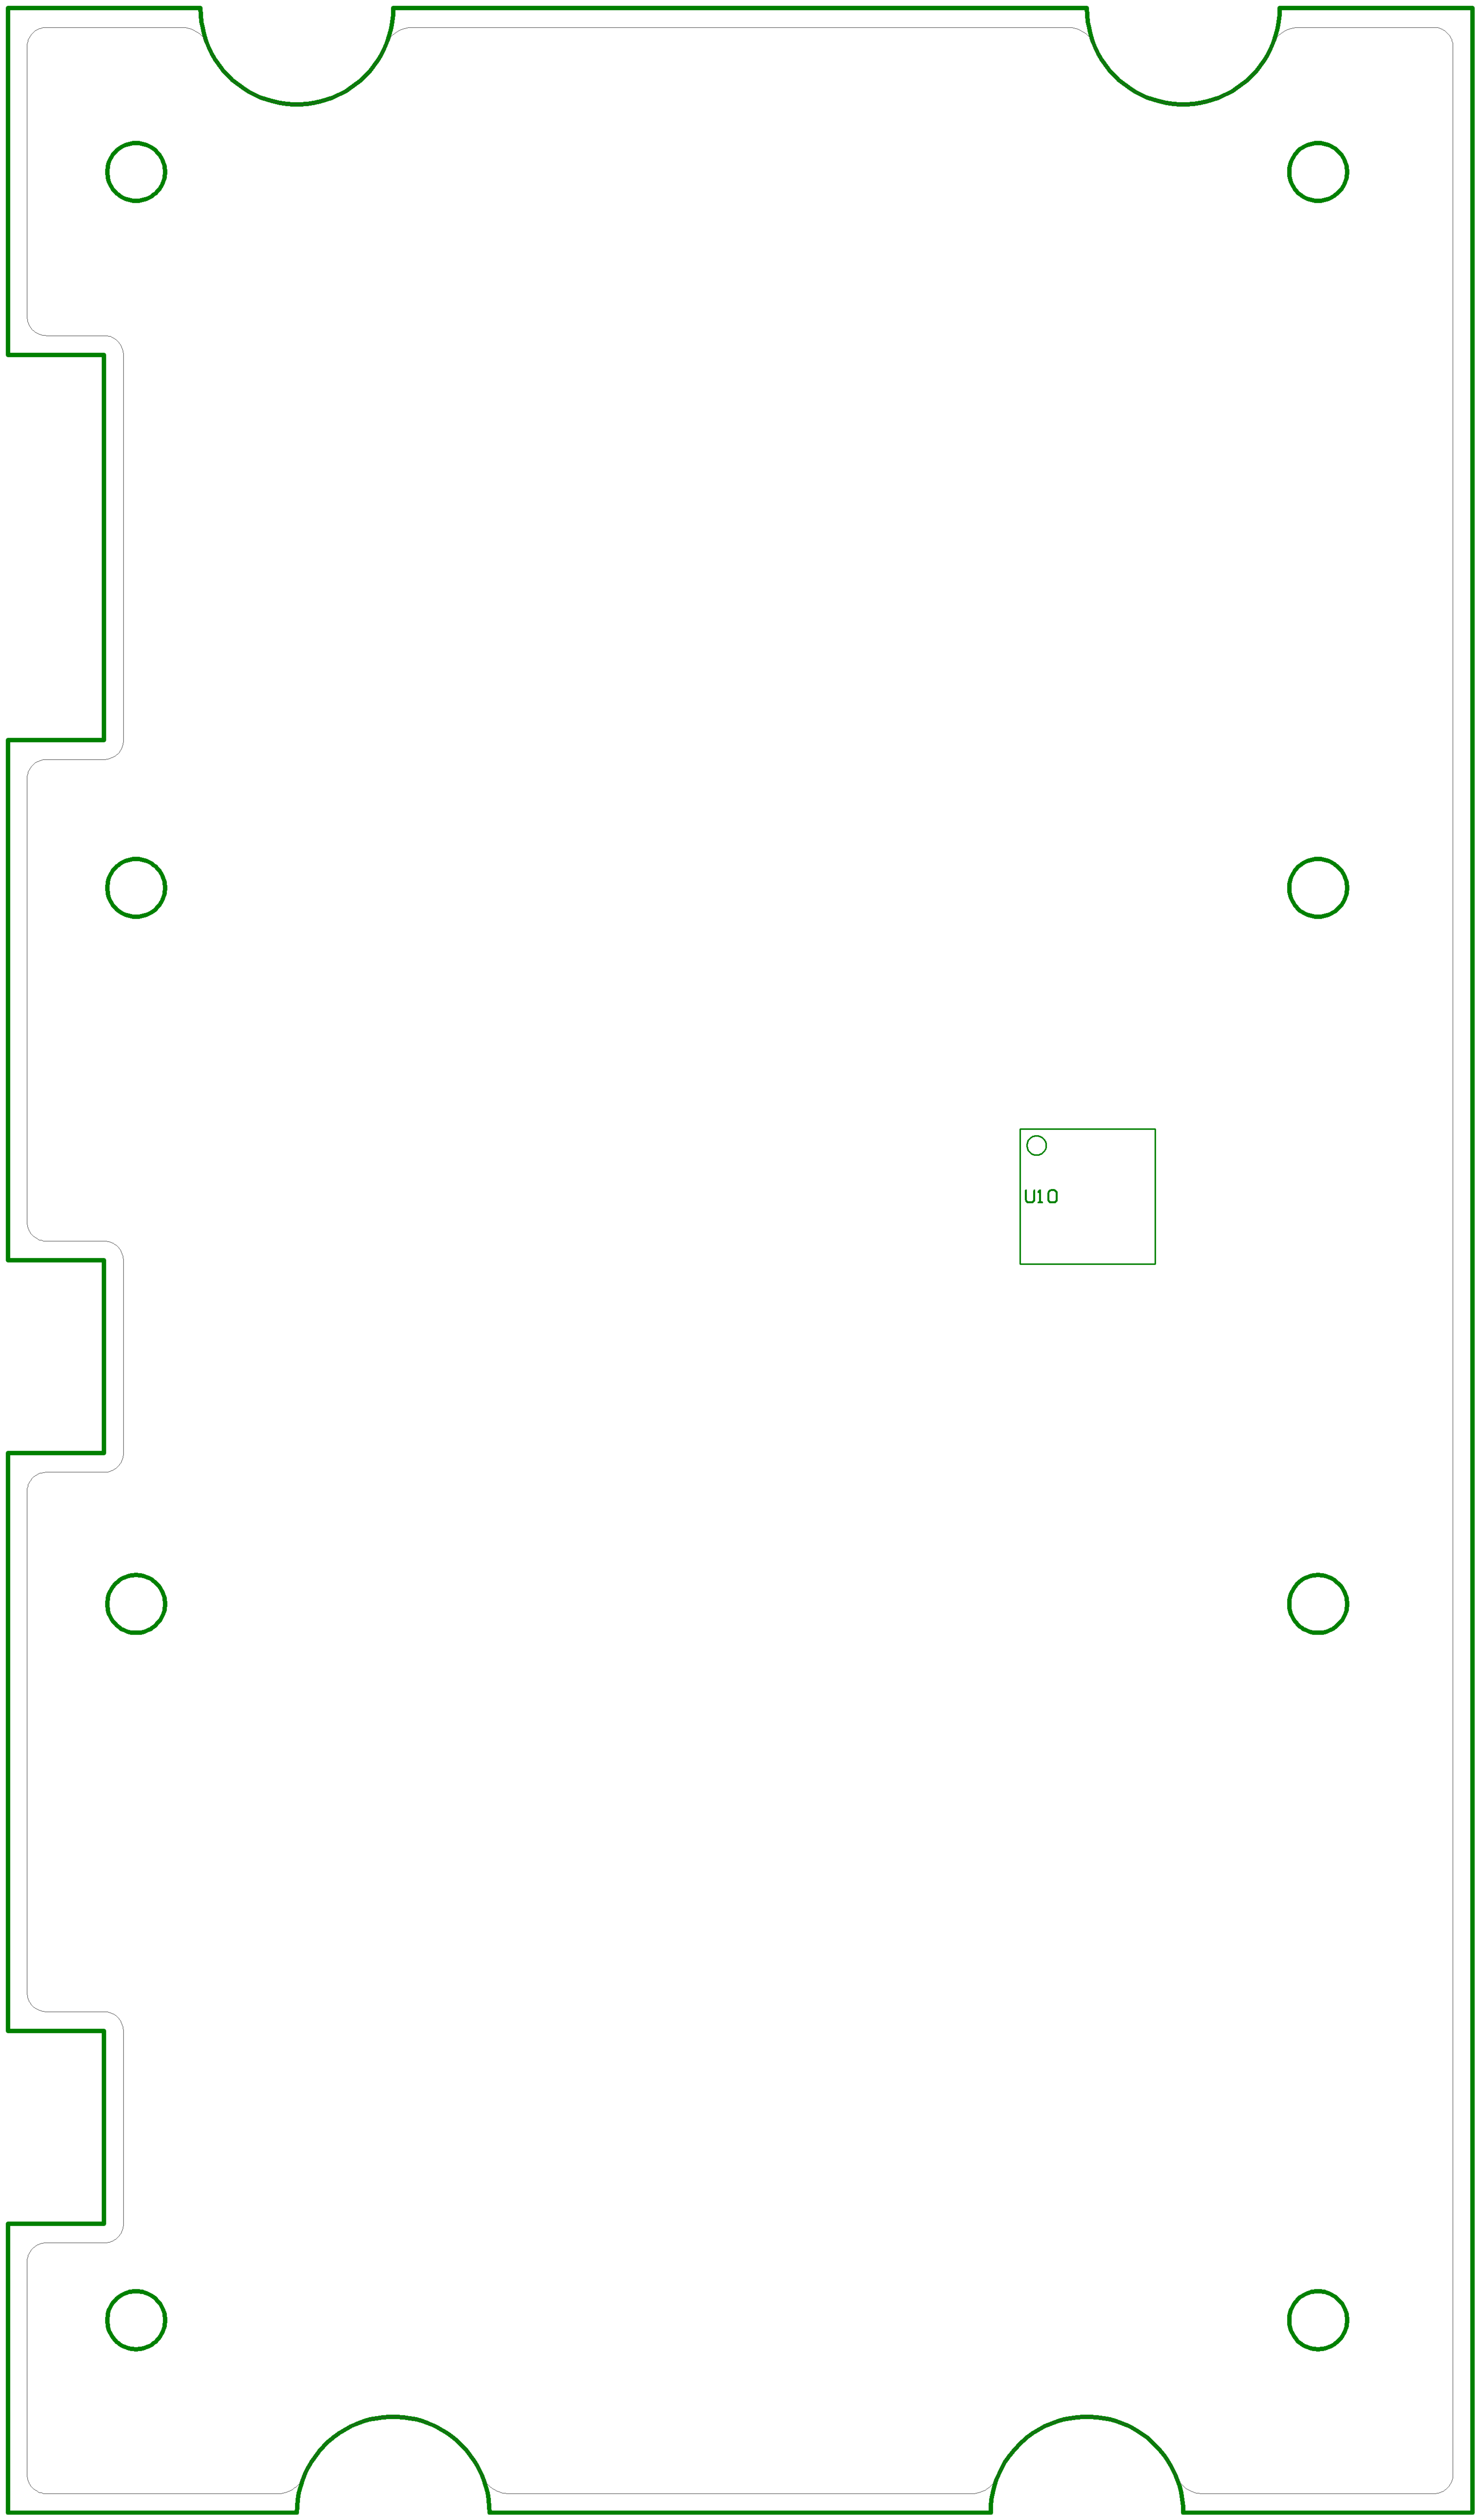
\includegraphics[width=\SmallSchematicWidth]{\Images/PCB/shape.eps}
    \caption{Board outlines}\label{img:board_shape}
\end{figure}

In green, and with right angles, there the exported shape from the mechanical
conception. We defined a bit smaller board shape than that, to ensure that the
manufacturing tolerances wont cause any issues, and to add some margin. This
final board shape \ref{img:board_shape} is not clearly visible on the image, as
it's drawn in grey and on a thin line.

There's a lot of mechanical support, by both screws and cuts to ensure the
board can't be mounted backward. This is required to ensure the positing system
has always the same reference position.

And, to finish, there some cutouts on the left side, to let more space for
wirings. Thus, we can easily make wires runs from the engines to the board
without damaging them.

\FloatBarrier

\subsection{Floorplan}
From all of these settings, we can establish a first floorplan. As there is
some cutouts for wires on the board, the position of some connectors /
soldering pads needs to be defined, to ensure the wire won't need to go
throught the board ! But there are lot of others elements with a defined
position, these includes :

\begin{itemize}[noitemsep]
    \item   Antennas and related ICs / passives (needs to be really close to the source,
          with excellent grounding)
    \item   Position of the accelerometers (Placed on two opposite corners of the board).
    \item   Position of the IMU, which shall be placed near the center of the board, to
          prevent rotational aberations and misalignement.
\end{itemize}